\documentclass[[table,border=3mm]{standalone}
\usepackage{tikz}
\usetikzlibrary{positioning}
	
\usepackage{xcolor}
\definecolor{lightgray}{gray}{0.9}
\begin{document}
\begin{tikzpicture}
\node (figure) at (0,0) {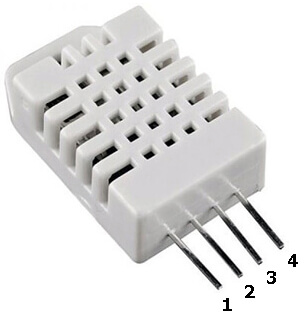
\includegraphics[scale=0.25]{DHT22.jpg}};
\node (tabular)[below = of figure] {\begin{tabular}{l|l}
\textbf{Pin} & \textbf{Funktion}\\ \hline \hline
1 & Betriebsspannung (3,3V - 5,5V) \\ \hline
2 & Serial Data Line\\\hline
3 & Nicht belegt\\ \hline
4 & Ground 
\end{tabular}};
\end{tikzpicture}
\end{document} 